\section{Triển khai DFS dạng lặp}

Đây là phần cốt lõi để xử lý flood fill. Thay vì dùng DFS đệ quy (dễ gây lỗi RecursionError), hệ thống sử dụng DFS dạng lặp với Stack.

Thuật toán \texttt{\_dfs\_reveal(start\_r, start\_c)} hoạt động theo các bước:

\textbf{Bước 1: Khởi tạo}  
Tạo một Stack (dùng list của Python) và đẩy ô bắt đầu vào.

\textbf{Bước 2: Vòng lặp LIFO}  
Trong khi Stack chưa rỗng, lấy phần tử trên cùng ra bằng \texttt{pop()}, gọi là $(cr, cc)$.

\textbf{Bước 3: Kiểm tra hợp lệ}  
Bỏ qua ô nếu:
\begin{itemize}
    \item Đã mở (\texttt{revealed == True})
    \item Đang bị cắm cờ (\texttt{flagged == True})
\end{itemize}

\textbf{Bước 4: Cập nhật trạng thái}  
Đánh dấu ô hiện tại là đã mở: \texttt{revealed[cr][cc] = True}.

\textbf{Bước 5: Quyết định mở rộng}  
Dựa vào giá trị \texttt{neighbour[cr][cc]}:
\begin{itemize}
    \item Nếu bằng 0: tiếp tục duyệt 8 ô lân cận. Ô hợp lệ sẽ được đẩy vào Stack để xử lý tiếp.
    \item Nếu lớn hơn 0: đây là ô viền. Thuật toán dừng lan theo nhánh này (backtracking).
\end{itemize}

Quá trình lặp lại cho đến khi Stack rỗng, nghĩa là toàn bộ vùng liên thông đã được mở. Nhờ cách triển khai này, flood fill đạt hiệu năng tuyến tính $O(N)$ và không gặp giới hạn đệ quy.

Vì mỗi ô chỉ được đánh dấu đã thăm một lần, tổng chi phí duyệt bị chặn trên bởi số đỉnh của đồ thị, dẫn đến độ phức tạp tuyến tính $\mathcal{O}(N)$. Phân tích chi tiết được trình bày trong Chương~\ref{chap:results}.

\begin{center}
\begin{figure}[H]
    \centering
    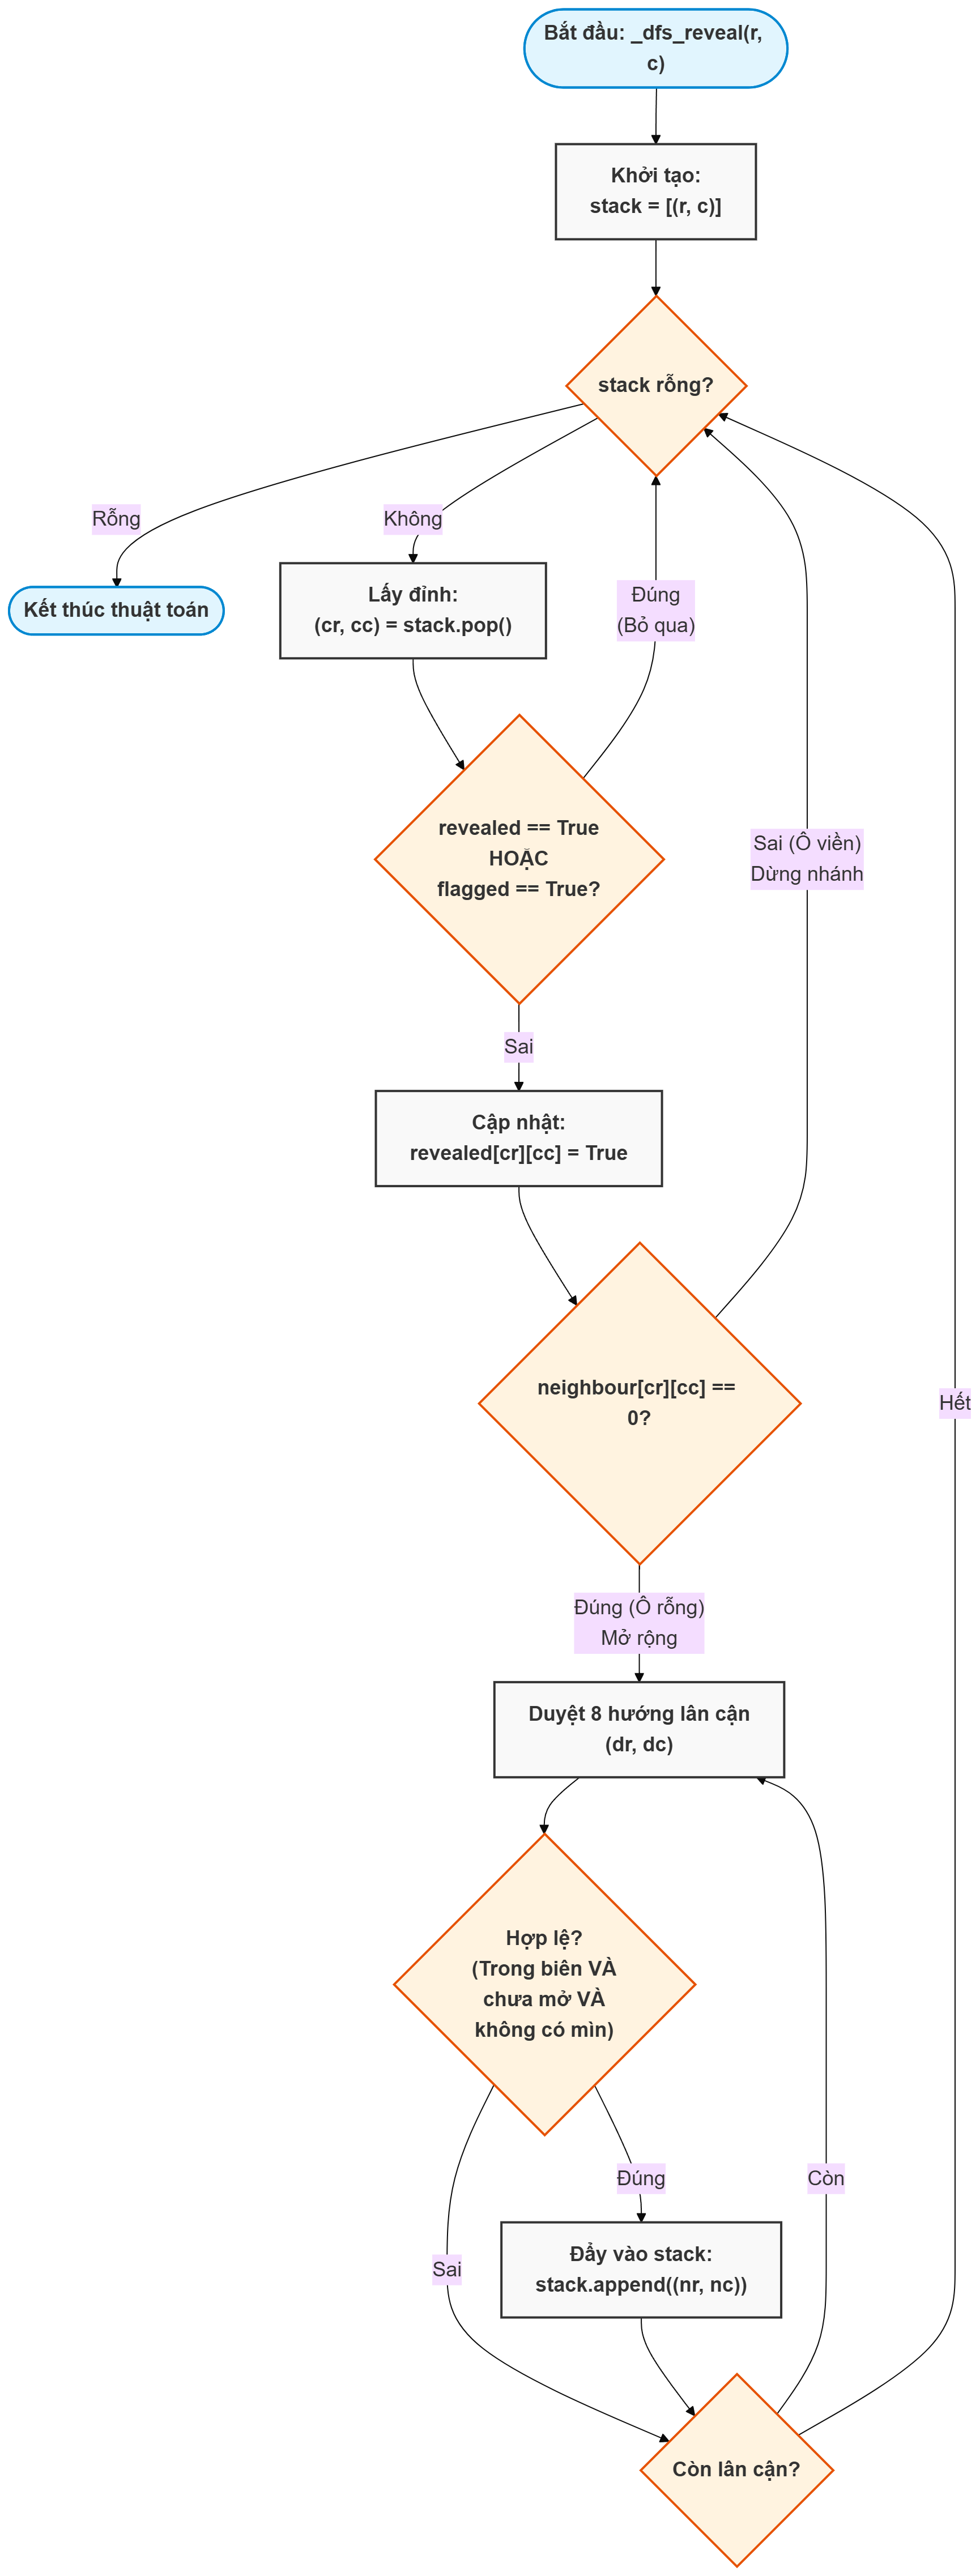
\includegraphics[width=0.5\linewidth]{../../images/ai/dfs_reveal.png}
    \vspace{0.5cm}
    \caption{Flowchart cho thuật toán \texttt{\_dfs\_reveal(start\_r, start\_c)}}
\end{figure}
\end{center}

\begin{algorithm}
\caption{Pseudocode cho thuật toán \texttt{\_dfs\_reveal(start\_r, start\_c)}}
\label{alg:dfs_reveal}
\begin{algorithmic}[1]
\Procedure{DFS-Reveal}{$r, c$}
    \State stack $\gets [(r, c)]$
    \While{stack is not empty}
        \State $(cr, cc) \gets$ stack.pop()
        \If{revealed[$cr$][$cc$] = true}
            \State \textbf{continue}
        \EndIf
        \If{flagged[$cr$][$cc$] = true}
            \State \textbf{continue}
        \EndIf
        \State revealed[$cr$][$cc$] $\gets$ true
        \If{neighbour[$cr$][$cc$] = 0}
            \For{$dr \in \{-1,0,1\}$}
                \For{$dc \in \{-1,0,1\}$}
                    \If{$dr \neq 0$ \textbf{or} $dc \neq 0$}
                        \State $(nr, nc) \gets (cr+dr, cc+dc)$
                        \If{Valid($nr, nc$) \textbf{and} not revealed[$nr$][$nc$] 
                        \textbf{and} not mine[$nr$][$nc$]}
                            \State stack.push($(nr, nc)$)
                        \EndIf
                    \EndIf
                \EndFor
            \EndFor
        \EndIf
    \EndWhile
\EndProcedure
\end{algorithmic}
\end{algorithm}



